\chapter{Early Exiting}

Early exiting have shown promising result in \cite{teerapittayanon_branchynet:_2016, teerapittayanon_distributed_2017, huang_multi-scale_2017}. Early exiting relies on the assumption, that the majority of samples are easy to classify correctly. \gls{dnn}s have become deeper to accurately classify the more difficult samples.

\begin{figure}
	\captionsetup[subfigure]{justification=centering}
	\centering
	\subfloat[bluetick]{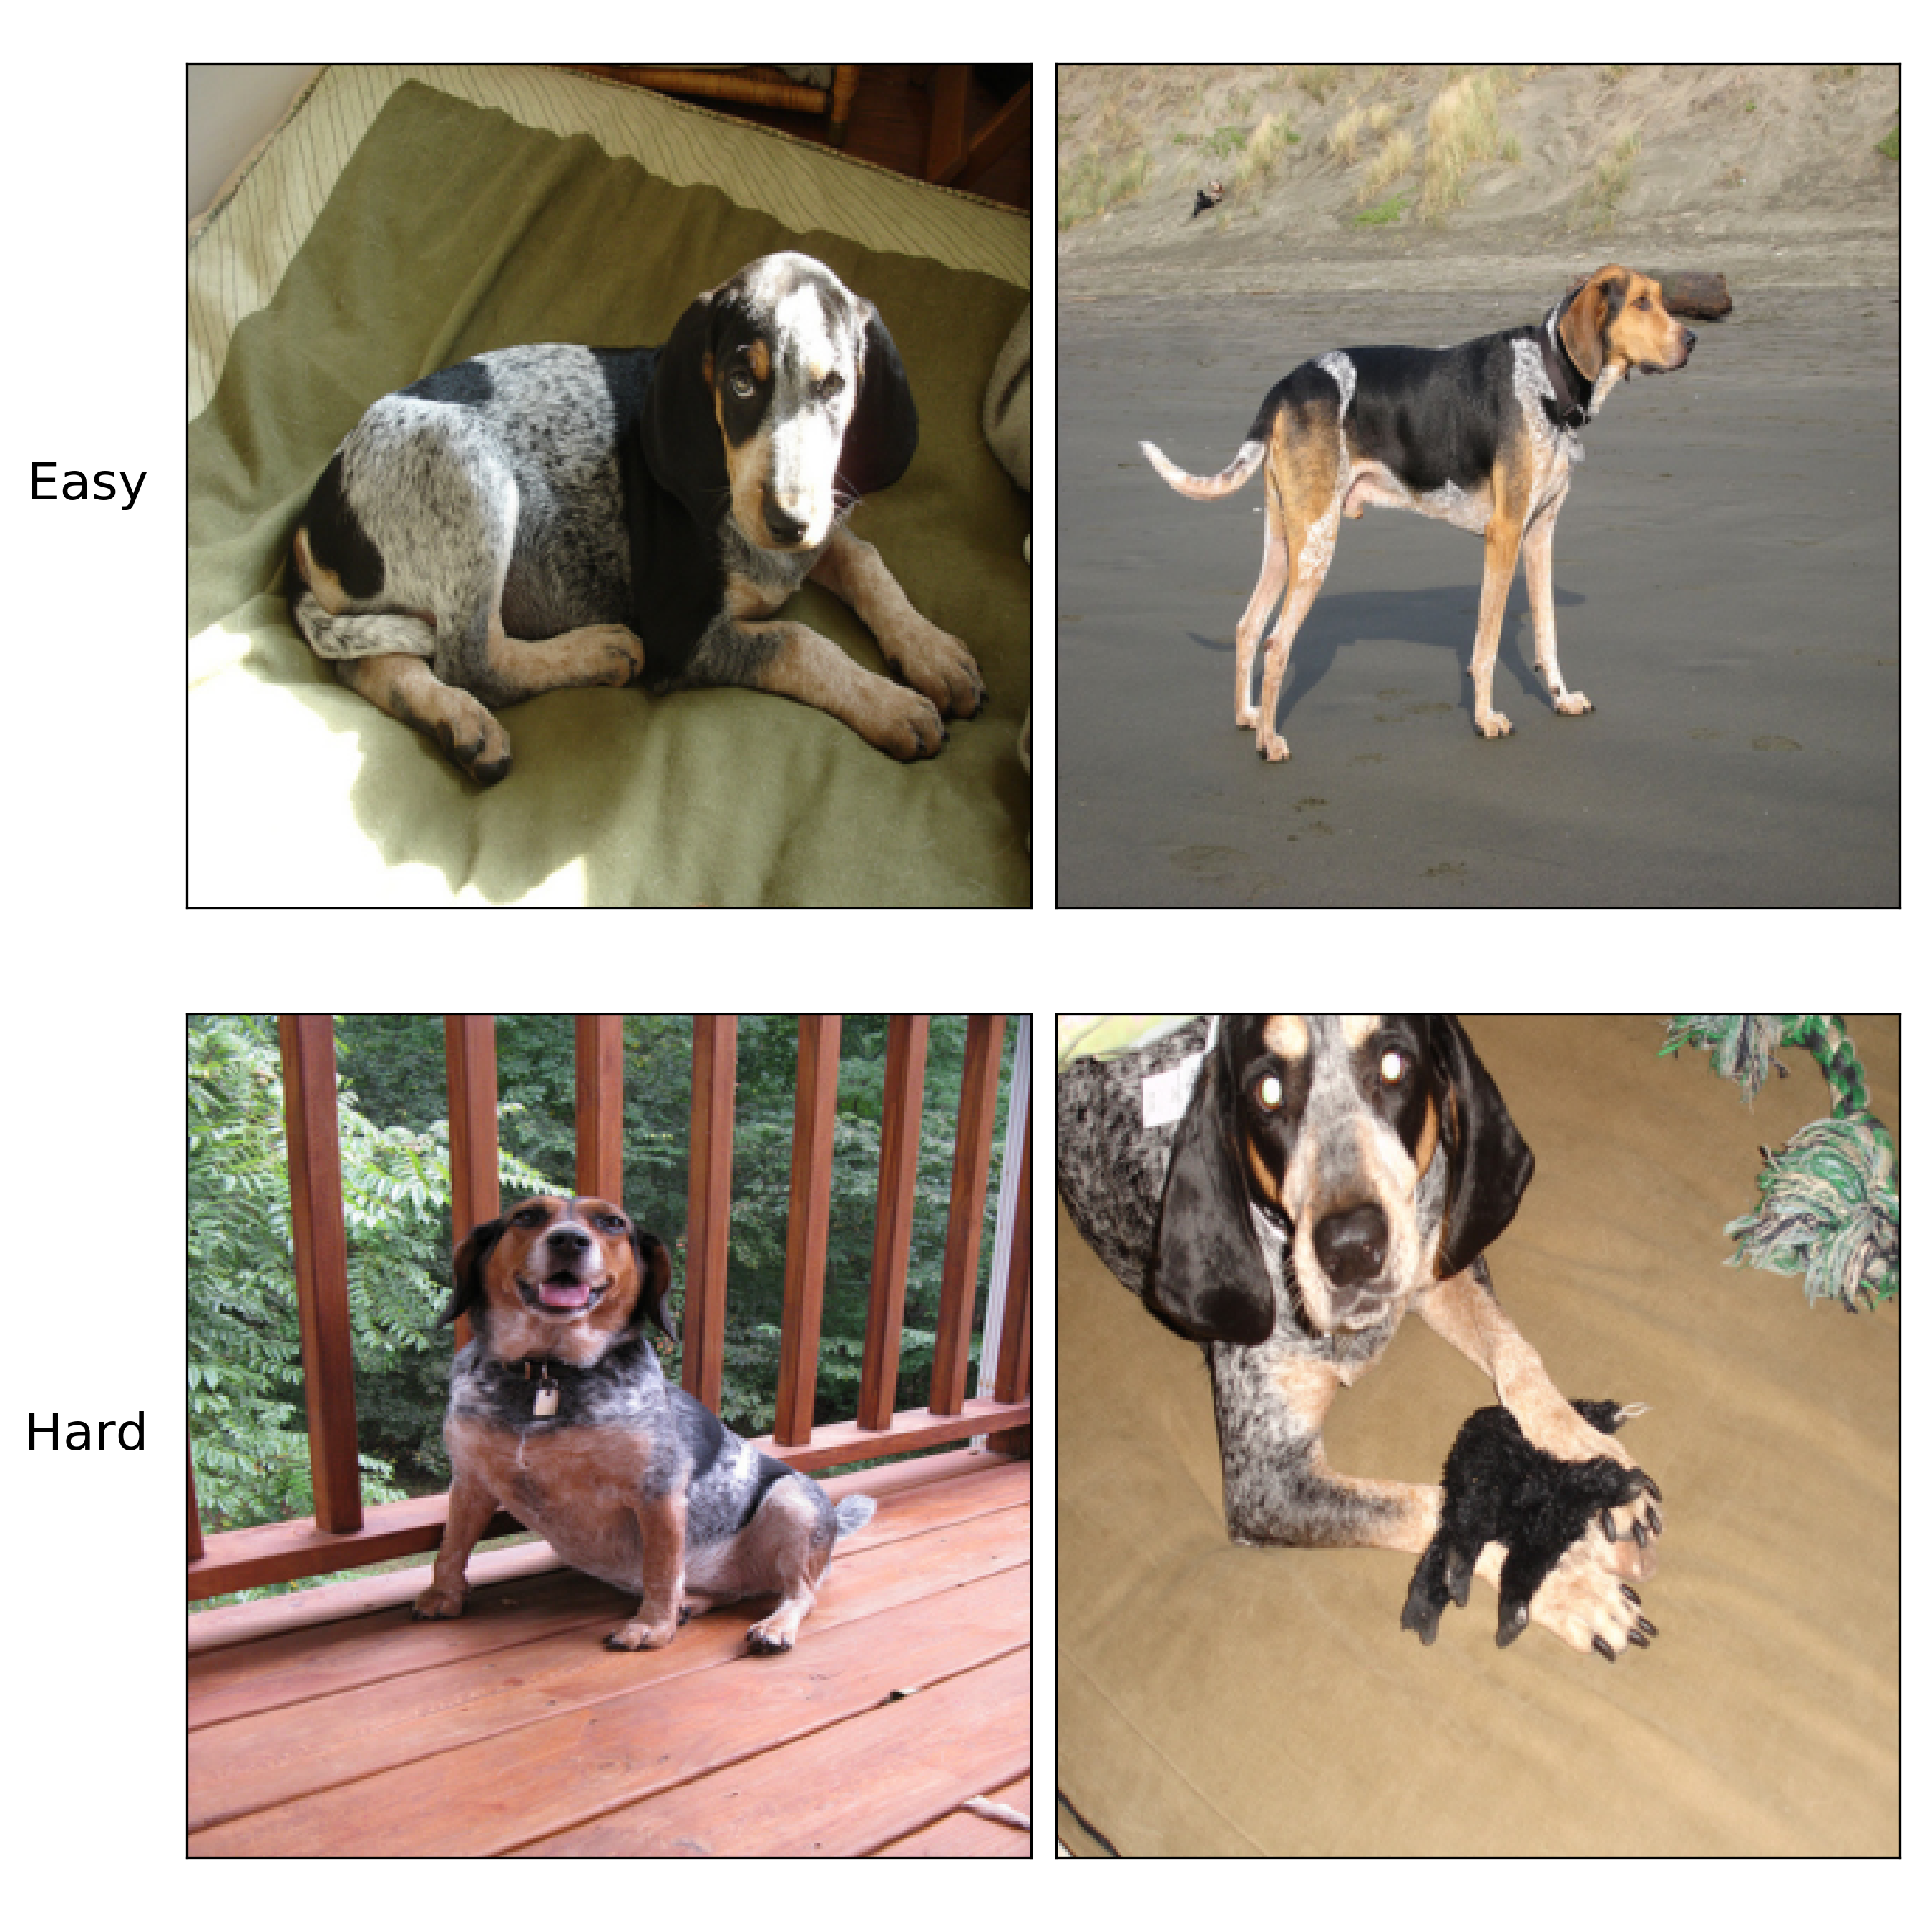
\includegraphics[width=0.5\linewidth]{figures/illustrations/hard_vs_easy_dog}}
	\subfloat[flamingo]{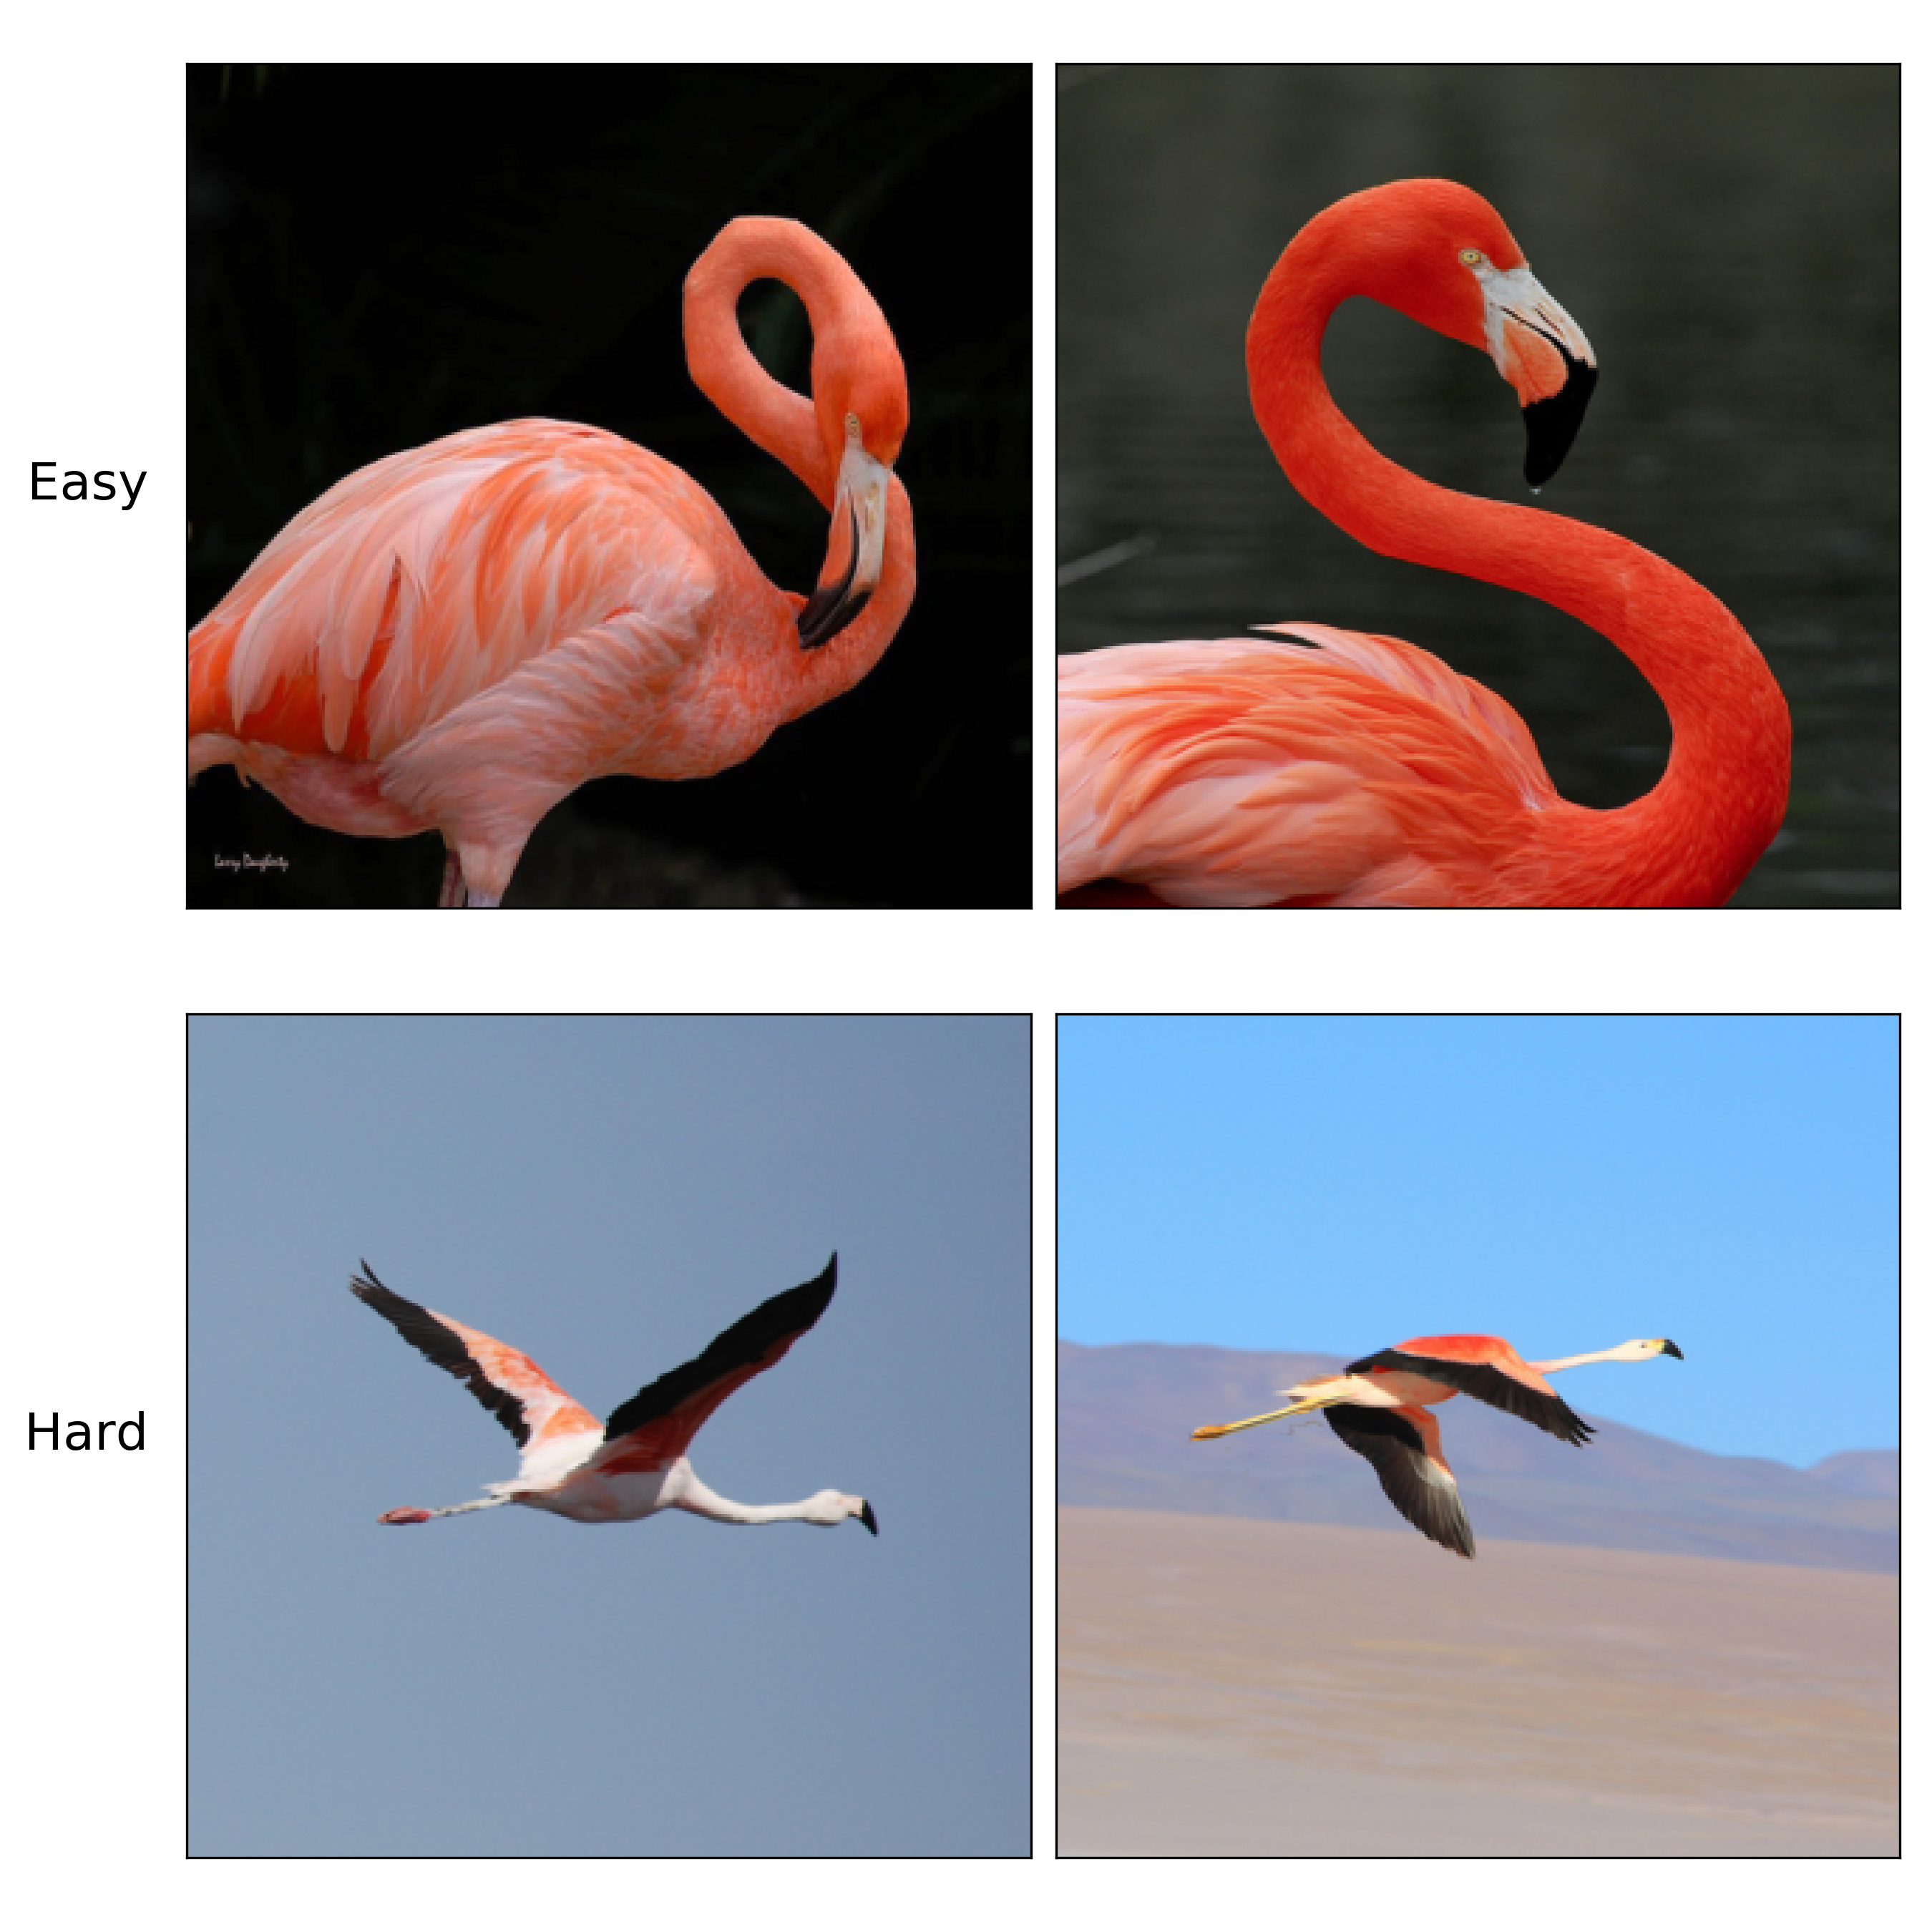
\includegraphics[width=0.5\linewidth]{figures/illustrations/hard_vs_easy_flamingo}}
	\caption[Easy vs. Hard Samples]{Easy vs. Hard Samples}
	\label{fig:hardvseasydog}
\end{figure}



\gls{branchynet} \cite{teerapittayanon_branchynet:_2016} is framework  for existing \gls{dnn}s, that allow samples, that can be classified earlier to exit the model, hence reducing the latency of computing all layer of the network.

\section{BranchyNet}

\begin{figure}
	branchynet framework
\end{figure}

Proposed by \citeauthor{teerapittayanon_branchynet:_2016} \gls{branchynet} \cite{teerapittayanon_branchynet:_2016} is a method to reduce inference latency by letting samples, that can be classified early on exit the model.

\paragraph{BranchyNet Training Framework}

The network is trained solving the joint-optimization problem is defined as the weighted sum of each branch-prediction.

\begin{align*}
L(\hat{\mathbf{y}},\mathbf{y};\theta) = \sum_{n=1}^{N} w_m L(\hat{\mathbf{y}}_{exit_n},\mathbf{y};\theta)
\end{align*}

Where the loss function is the softmax cross-entropy objective.
The weighted sum loss is back-propagated to optimize the weights of the network. 

The paper uses the \gls{mnist} and \gls{cifar10} datasets for benchmarking. One may argue, that the two datasets used for benchmarking are not applicable to real-life scenarios, as the images are only 32x32 pixels and the datasets only contain 10.000 samples. This thesis studies BranchyNet on state-of-the-art \gls{dnn} \gls{resnet}50 and \gls{densenet}-121 on a subset of the ImageNet dataset. \gls{ilsvrc2012} contains 1.2 million images with an average size of 400 $\times$ 350 pixels.

Our assumption is running a model on device up to a certain exit, if the model can classify with high enough confidence, the sample is exited. However, if confidence is too poor, the intermediate result is offloaded to an edge server to perform final classification.  

\subsection{Branchy-ResNet}

In this section the design of Branchy-\gls{resnet} is explained. First is the building blocks of a residual network explained followed by the design of B-\gls{resnet}. 

Depth of \gls{dnn} is of paramount importance to extract increasingly richer features from images to obtain highly accurate classification models cite{who}. Training very deep models with more than ten layer for convergence is not easy due to vanishing/exploding gradients. Residual Networks or \gls{resnet} \cite{he_deep_2015} have for long been the state-of-the-art network and won ILSVRC15 using 152 layers. The network is build of residual blocks, a novel \gls{dnn} layer designed for extremely deep networks. 

Instead of simply stacking convolutional layers as plain \gls{vgg} nets, residual network adds a shortcut connection, which skip a layer or a block of layers. The skip connection adds the identity of input to the output of the layers/block, see figure \ref{fig:residualblock}

\begin{figure}
	\centering
	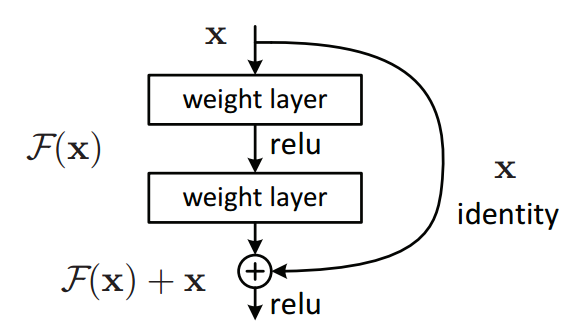
\includegraphics[width=.5\linewidth]{figures/models/residualblock}
	\caption[Residual Block]{Residaul Block}
	\label{fig:residualblock}
\end{figure}

Information from earlier layers are preserved by the residual, which diminishes the vanishing gradient problem. Thus this type of network have shown to be easier to train compared to it’s plain counterpart and able to obtain superior accuracy.  

Very deep residual networks comprised of up to 152 layers have also shown to be far more efficient requiring less \gls{flop}s, than \gls{vgg}16 comprised of only 16 layers, by introducing a bottleneck unit. The bottleneck reduces the dimensions by a $1 \times 1$ convolution, followed by a $3 \times 3$ convolution and then restoring the dimensions using a $1 \times 1$ convolution. 

The residual layers proposed in \cite{he_deep_2015} are grouped into 4 resolutions block with different number of layers (18, 34, 50, 101, 152) depending on the depth of the network. \gls{pytorch} provide implementations of these network. The networks can be trained from scratch or pretrained weights based on ImageNet can be downloaded. \gls{resnet}101 have been chosen for this project, as it has comparable depth to the smallest available \gls{pytorch} \gls{densenet}121 implementation and weights and also have roughly equal inference latency on a Titan Xp (8.90ms and 8.93ms) \cite{bianco_benchmark_2018}.


The architecture is further divided into 4 resolution blocks, each of which downsamples the input data. Table \ref{tbl:resnet50} describes the block and layers of the \gls{resnet} architecture. 

\pagebreak
\begin{longtabu}{>{\bfseries}X|X[c]|X[2c]}
	\caption[\gls{resnet}50 description]{\gls{resnet}50 description. The table describes the blocks of \gls{resnet}50, the size of the block and the layers of the block.} \label{tbl:resnet50} \\
	\toprule
	\rowfont{\bfseries}
	Resolution block & Output size & Layer description \tabularnewline
	\hline
	\endfirsthead
	\multicolumn{3}{@{}l}{\textbf{\textcolor{black}{Table \ref{tbl:resnet50}:}} continued}\\
	\toprule
	\rowfont{\bfseries}
	Conv block & Output size & Layer description \tabularnewline
	\hline
	\endhead % all the lines above this will be repeated on every page
	\hline
	\multicolumn{3}{@{}l}{continued \ldots}\\
	\endfoot
	\hline
	\endlastfoot
	conv1 & $112\times 112$& $7\times 7, 64, \:\mathrm{stride}\: 2$ \tabularnewline \hline
	
	\multirow{5}{*}{conv2\_x} 	& \multirow{5}{*}{$56 \times 56$} 	& $3 \times 3 \:\mathrm{maxpool, stride}\: 2 $ \\ \tabucline{3-3} & & \multirow{4}{*}{
		$\begin{bmatrix}
		1 \times 1, 64 \\ 3 \times 3, 64 \\1 \times 1, 256
		\end{bmatrix} \times 3$ }		\tabularnewline										
	& & 	\tabularnewline
	& & 	\tabularnewline
	& & 	\tabularnewline
	\hline
	
	\multirow{4}{*}{conv3\_x} 	& \multirow{4}{*}{$28\times 28$} & \multirow{4}{*}{
		$\begin{bmatrix}
		1 \times 1, 128 \\ 3 \times 3, 128 \\1 \times 1, 512
		\end{bmatrix} \times 4$ }		\tabularnewline										
	& & 	\tabularnewline
	& & 	\tabularnewline
	& & 	\tabularnewline
	\hline
	
	\multirow{4}{*}{conv4\_x} 	& \multirow{4}{*}{$14\times 14$} & \multirow{4}{*}{
		$\begin{bmatrix}
		1 \times 1, 256 \\ 3 \times 3, 256 \\1 \times 1, 1024
		\end{bmatrix} \times 6$}		\tabularnewline										
	& & 	\tabularnewline
	& & 	\tabularnewline
	& & 	\tabularnewline
	\hline
	
	\multirow{4}{*}{conv5\_x} 	& \multirow{4}{*}{$7\times 7$} & \multirow{4}{*}{
		$\begin{bmatrix}
		1 \times 1, 512 \\ 3 \times 3, 512 \\1 \times 1, 2048
		\end{bmatrix} \times 3$}		\tabularnewline										
	& & 	\tabularnewline
	& & 	\tabularnewline
	& & 	\tabularnewline
	\hline
	
	Classifier & \multicolumn2{c}{$\mathrm{Avg.\: Pool,\:} 1000d\: \mathrm{fc,\: Softmax}$} \tabularnewline
	\bottomrule
\end{longtabu}
\vspace{-20pt} \color{caption-color}{\textit{Source: \citetitle{he_deep_2015}, by \citeauthor{he_deep_2015} \cite{he_deep_2015}, describes a full list of Residual Networks (\gls{resnet}18, \gls{resnet}34, \gls{resnet}50, \gls{resnet}101 and \gls{resnet}152)}}\color{main-color}

The early exits of Branchy-\gls{resnet}50 is placed immediately after a resolution block, as 1) we have to go deep enough, that the model is actually able to correctly predict some input samples. 2) we wish a smaller representation of the input and within a resolution block the data size is unchanged. Hence if offloading after a resolution block 2) is fulfilled and we must by experiment determine how deep within the model exits should be in order to classify some portion of input.

For each exit, the intermediate features are fed to a pooling-layer and a fully-connected softmax classifier. If the output of the  softmax classifier is acceptable the sample is exited. Figure \ref{fig:b-resnet} visualizes the early exiting model B-\gls{resnet}50.

\begin{figure}
	\centering
	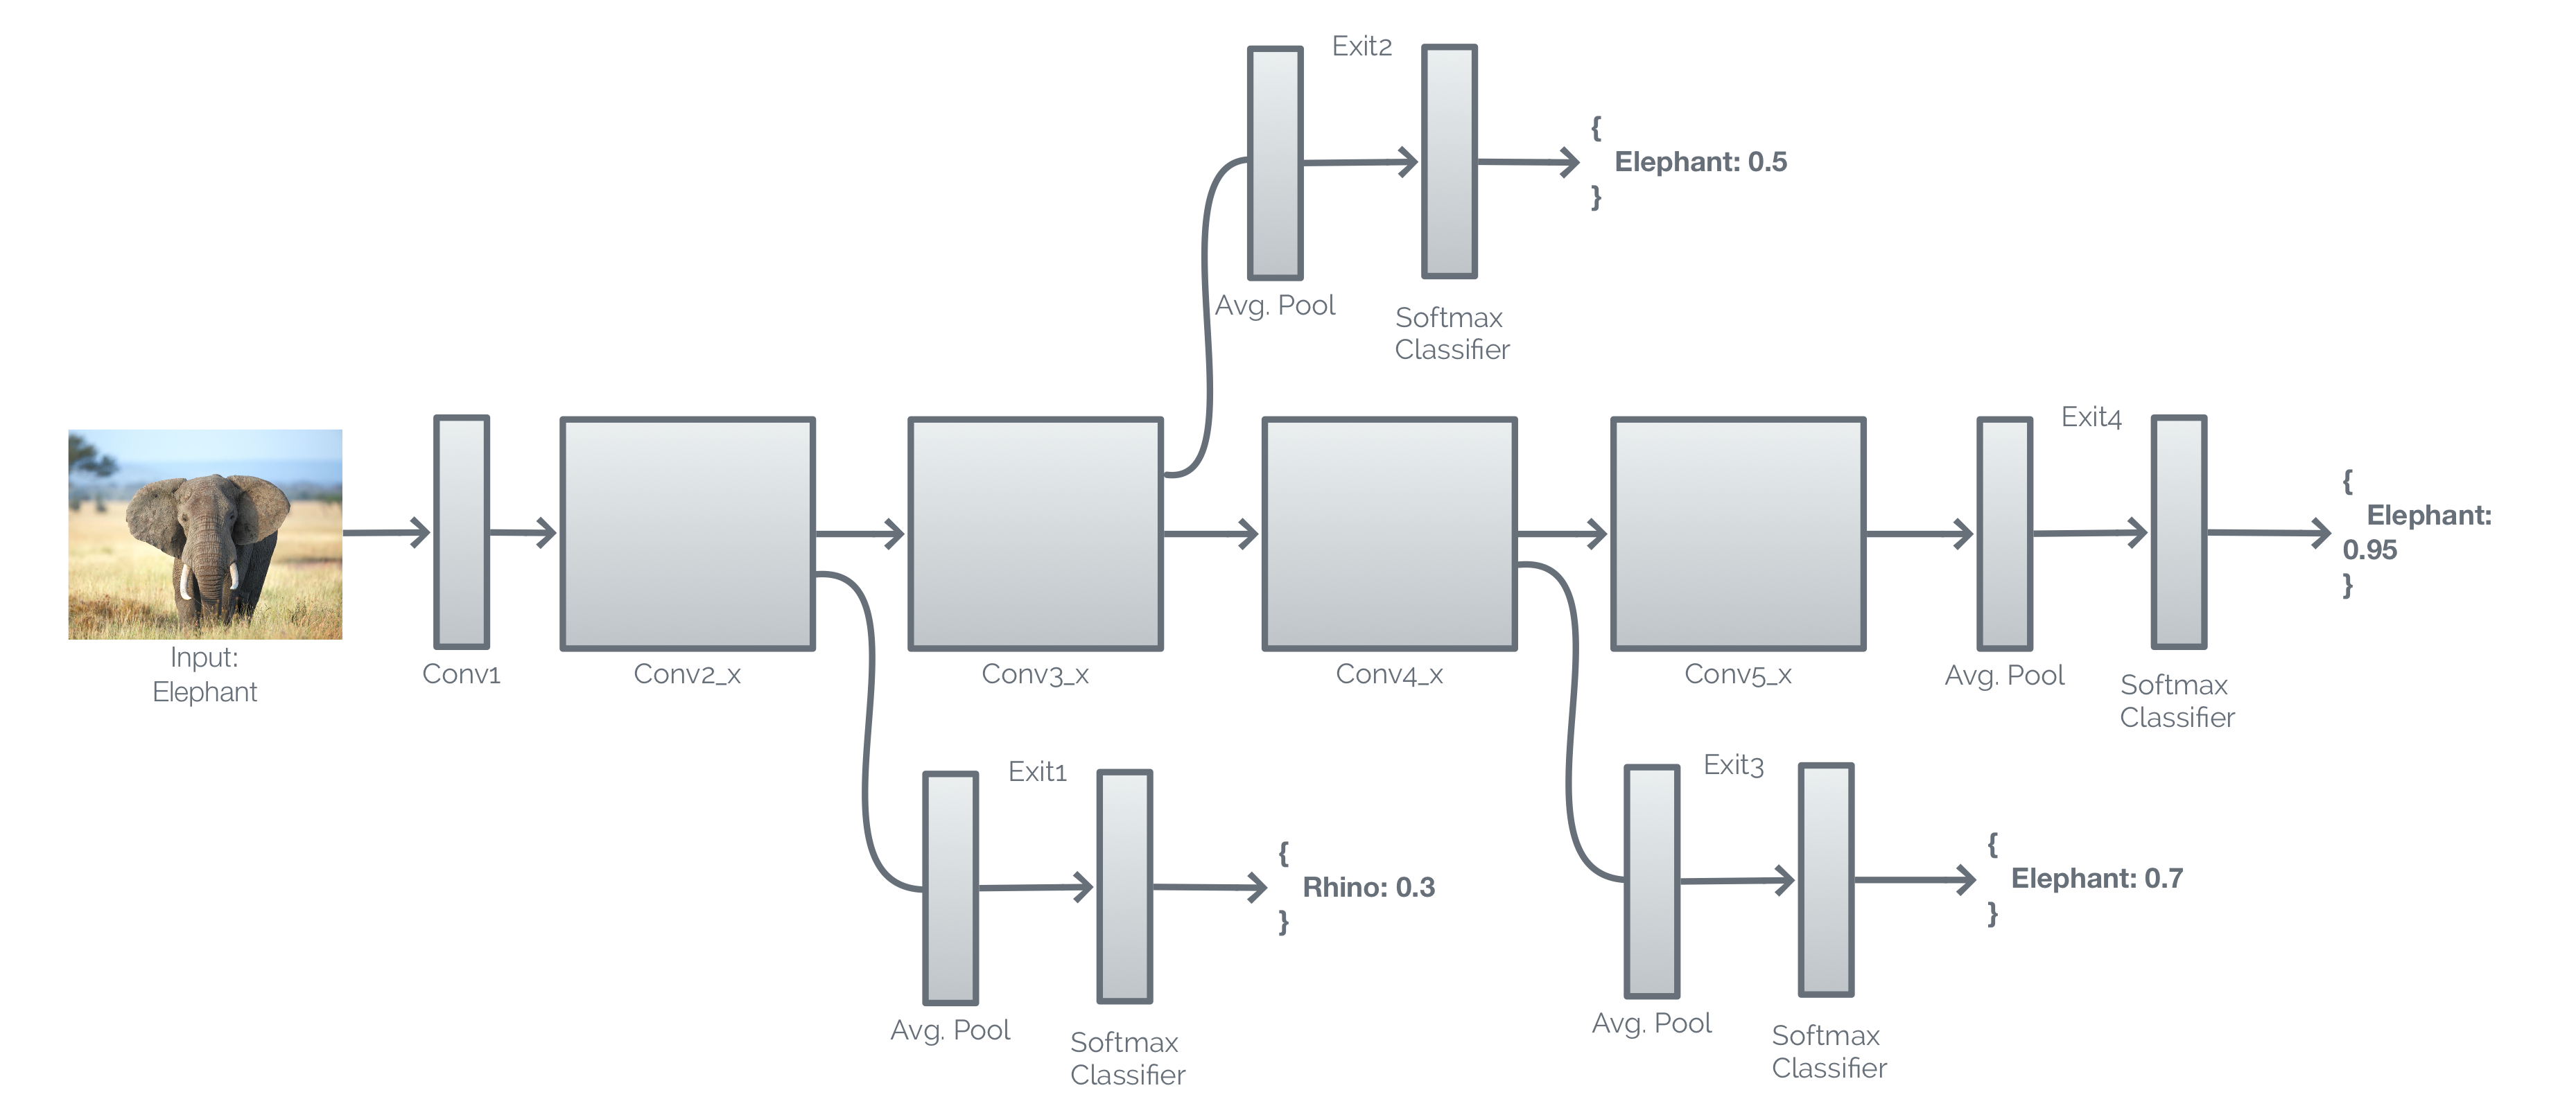
\includegraphics[width=\linewidth]{figures/models/BResNet}
	\caption[B-\gls{resnet} architecture]{Branchy-\gls{resnet}50: \gls{resnet}50 extended to implement the BranchyNet framework. The figure illustrates how classification confidence grows, as we go deeper in the model. The first exit actually fails to classify the elephant. }
	\label{fig:b-resnet}
\end{figure}


\subsection{Branchy-DenseNet}

In this section the design of Branchy-\gls{densenet} is explained. First is the building blocks of a dense network explained followed by the design of B-\gls{densenet}.

DenseNet \cite{huang_densely_2016} is build on the assumption, that many layers of \gls{resnet} have only a small contribution to the output and can in fact be dropped during training \cite{huang_densely_2016}. Instead of adding previously learned information to the output, \gls{densenet} combines features from all subsequent layers by concatenation, as there is no need to relearn redundant information. Figure \ref{fig:denseblock} show the dense connections, that combine features from previous layers and show how the features size grows throughout a densely connected block

\begin{figure}
	\centering
	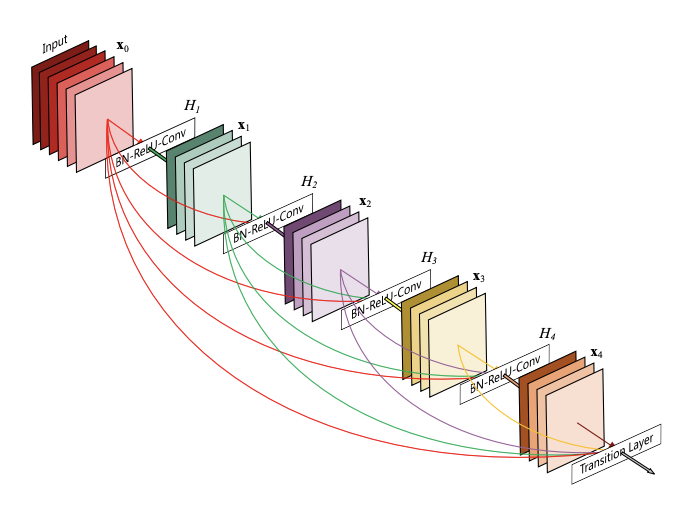
\includegraphics[width=.5\linewidth]{figures/models/denseblock}
	\caption[Densely Connected Block]{Densely Connected Block}
	\label{fig:denseblock}
\end{figure}

The densely connected layers are likewise residual network grouped into resolution block called dense blocks, but for \gls{densenet} intermediate transition layers are added between dense block to downsample the feature size. 

\begin{figure}
	\centering
	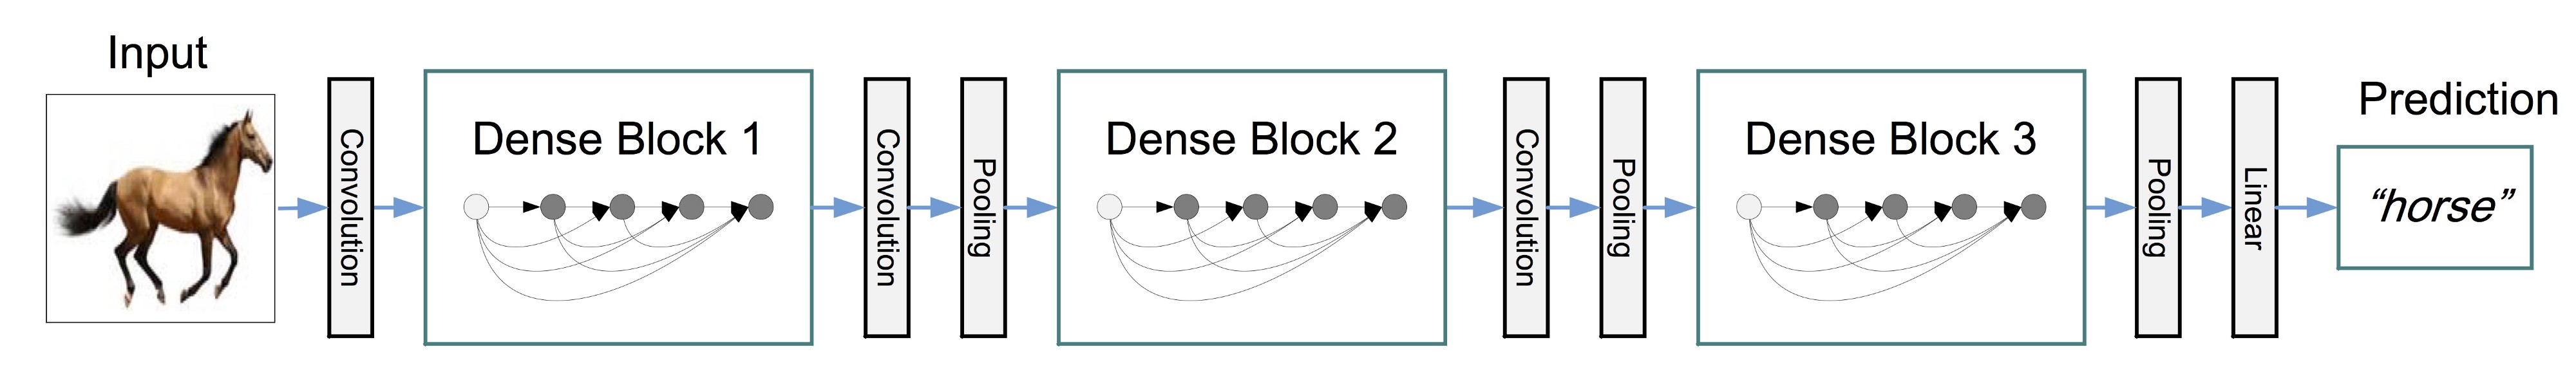
\includegraphics[width=\linewidth]{figures/models/densenet}
	\caption[Densely Connected Block]{Densely Connected Block}
	\label{fig:densenet}
\end{figure}

The collective knowledge from all preceding layers gives more diversified features compared to the correlated features of \gls{resnet}s. In \cite{huang_multi-scale_2017} the diversified features are shown to be more suited for early exiting,  as the information are better preserved using dense connection, hence even though information may have been collapsed to generate a short-term feature for the classifier. Thus placement of an intermediate classifier have less impact on the learned features for a later classifier. \gls{densenet} can be thinner as the number of channel can be fewer, thus more efficient compared to traditional and residual networks. Additionally densely connected blocks have a regularizing effect thus reducing overfitting the training data, hence perform better on smaller training sets. 

Table \ref{tbl:densenet121} describes the block and layers of the \gls{densenet} architecture. 

\pagebreak
\begin{longtabu}{>{\bfseries}X|X[c]|X[2c]}
	\caption[\gls{densenet}-121 description]{\gls{densenet}-121 description. The table describes the blocks of \gls{densenet}-121. $k$ is the growth rate of the DenseBlock. A typical setting is $k=32$ yielding 256, 512 and 1024 output channels for denseblock(1-3) respectively. The transition layer downsamples the output channel by a factor of 2, thus the number of input channels for DenseBlock(2-4) becomes 128, 256 and 512 respectively.} \label{tbl:densenet121} \\
	\toprule
	\rowfont{\bfseries}
	Layers & Output size & Layer description \tabularnewline
	\hline
	\endfirsthead
	\multicolumn{3}{@{}l}{\textbf{\textcolor{black}{Table \ref{tbl:resnet50}:}} continued}\\
	\toprule
	\rowfont{\bfseries}
	Layers & Output size & Layer description \tabularnewline
	\hline
	\endhead % all the lines above this will be repeated on every page
	\hline
	\multicolumn{3}{@{}l}{continued \ldots}\\
	\endfoot
	\hline
	\endlastfoot
	Convolution & $112\times 112$& $7\times 7, \:\mathrm{stride}\: 2$ \tabularnewline \hline
	Pooling & $56\times 56$& $3\times 3, \:\mathrm{maxpool},\:  \mathrm{stride}\: 2$ \tabularnewline \hline
	\multirow{3}{*}{DenseBlock (1)} 	& \multirow{3}{*}{$56 \times 56$} & \multirow{3}{*}{
		$\begin{bmatrix}
		1 \times 1, k \\ 3 \times 3, k \\
		\end{bmatrix} \times 6$ }		\tabularnewline										
	& &  	\tabularnewline
	& & 	\tabularnewline
	\hline
	
	Transition  	& $56 \times 56$ & $1 \times 1\: \mathrm{conv}$ \tabularnewline \tabucline{2-3}							
	Layer (1) & $28\times 28$ & $2\times 2\: \mathrm{average\: pool,\: stride}\: 2$	\tabularnewline
	
	\hline
	
	\multirow{3}{*}{DenseBlock (2)} 	& \multirow{3}{*}{$28 \times 28$} & \multirow{3}{*}{
		$\begin{bmatrix}
		1 \times 1, k \\ 3 \times 3, k \\
		\end{bmatrix} \times 12$ }		\tabularnewline										
	& &  	\tabularnewline
	& & 	\tabularnewline
	\hline
	
	Transition  	& $28 \times 28$ & $1 \times 1\: \mathrm{conv}$ \tabularnewline \tabucline{2-3}							
	Layer (2) & $14\times 14$ & $2\times 2\: \mathrm{average\: pool,\: stride}\: 2$	\tabularnewline
	
	\hline
	
	\multirow{3}{*}{DenseBlock (3)} 	& \multirow{3}{*}{$14 \times 14$} & \multirow{3}{*}{
		$\begin{bmatrix}
		1 \times 1, k \\ 3 \times 3, k \\
		\end{bmatrix} \times 24$ }		\tabularnewline										
	& &  	\tabularnewline
	& & 	\tabularnewline
	\hline
	
	Transition  	& $14 \times 14$ & $1 \times 1\: \mathrm{conv}$ \tabularnewline \tabucline{2-3}							
	Layer (3) & $7\times 7$ & $2\times 2\: \mathrm{average\: pool,\: stride}\: 2$	\tabularnewline
	
	\hline
	
	\multirow{3}{*}{DenseBlock (4)} 	& \multirow{3}{*}{$7 \times 7$} & \multirow{3}{*}{
		$\begin{bmatrix}
		1 \times 1, k \\ 3 \times 3, k \\
		\end{bmatrix} \times 16$ }		\tabularnewline										
	& &  	\tabularnewline
	& & 	\tabularnewline
	\hline
	
	Classification  	& $1 \times 1$ & $7 \times 7\: \mathrm{global\: average\: pool}$ \tabularnewline \tabucline{2-3}							
	Layer &  \multicolumn2{c}{$\mathrm{Avg.\: Pool,\:} 1000d\: \mathrm{fc,\: Softmax}$} \tabularnewline
	\bottomrule
\end{longtabu}
\vspace{-20pt} \color{caption-color}{\textit{Source: \citetitle{huang_densely_2016}, by \citeauthor{huang_densely_2016} \cite{huang_densely_2016}, describes a full list of Densely Connected Networks (\gls{densenet}-121, \gls{densenet}-169, \gls{densenet}-201 and \gls{densenet}-264)}} \color{main-color}


In the same fashion as B-ResNet early exits have been placed to construct B-DenseNet. The exits are placed after a DenseBlock to obtain feature of sufficient quality and exiting as quickly as possible. If used in Edge-Device mode and the confidence was insufficient the transition layer after the DenseBlock is executed, before data is being preprocess for offloading. 

\section{MSDNet}

In contrast to the early exiting framework of \gls{branchynet} for any model comprised of stacking layers on top of each other, \gls{msdnet} \cite{huang_multi-scale_2017} is a \gls{dnn} specifically designed for early exiting. \gls{msdnet} takes advantage of densely connected layers and add multi-scale paths to further improve upon early exiting, see figure \ref{fig:msdnet}.

\begin{figure}
	\centering
	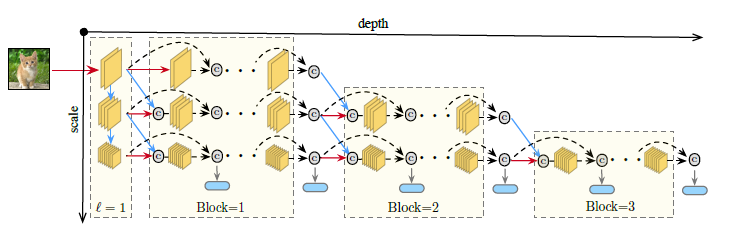
\includegraphics[width=\linewidth]{figures/models/msdnet}
	\caption[\gls{msdnet} Architecture]{\gls{msdnet} Architecture, Source: \citetitle{huang_multi-scale_2017} \cite{huang_multi-scale_2017}}
	\label{fig:msdnet}
\end{figure}

\gls{msdnet} addresses two main problems concerning early exiting. The first problem is the lack of coarse-level features in early classifiers. Traditional \gls{dnn}s uses stacking of layers to get coarse level features, which the early classifier lacks, thus giving unsatisfactory high error-rates. important for classification. Multi-scale feature maps addresses this issues by preserving high-resolution information and allow constructing coarse-level features for all classifiers in the network.

The second problem is early classifiers interfere with later classifiers. The early classifiers might cause early features to be optimized for the short-term by collapsing information prematurely,thus harming the later and final classifiers. Their study reveals, that densely connected layers suffers mush less from intermediate classifiers, as a layer is connected to all previous layer and is therefore able to recover collapsed information.


\section{Overall Comparison}


\begin{longtabu}{>{\bfseries}X|X[r]|X[r]|X[r]}
	\caption[Model Parametric Comparison]{Model Parametric Comparison using \texttt{thop} \cite{zhu_thop_nodate}. The test is conducted by inference a random 4d tensor of size $ (\mathrm{batch,channels,width,height})=(1,3,224,224) $ to all models.}  \label{} \\
	\toprule
	\rowfont{\bfseries}
	Model & Layers & Parameters (M) & G\gls{flop} \tabularnewline
	\hline
	\endfirsthead
	\multicolumn{3}{@{}l}{\textbf{\textcolor{black}{Table \ref{}:}} continued}\\
	\toprule
	\rowfont{\bfseries}
	Model & Layers & Parameters (M) & G\gls{flop} \tabularnewline
	\hline
	\endhead % all the lines above this will be repeated on every page
	\hline
	\multicolumn{3}{@{}l}{continued \ldots}\\
	\endfoot
	\hline
	\endlastfoot
	ResNet & $ 101 $ & $ 42.705 $ & $ 7.864 $ \tabularnewline
	\hline
	DenseNet & $ 121 $ & $ 7.056 $ & $ 2.897 $ \tabularnewline
	\hline
	B-ResNet & $ 107 $ & $ 42.885 $ & $ 7.866 $ \tabularnewline
	\hline
	B-DenseNet & $ 127 $ & $ 7.236 $ & $ 2.898 $\tabularnewline
	\hline
	MSDNet & $ 24 $ & $ 23.958 $ & $ 1.374 $ \tabularnewline
	\bottomrule
\end{longtabu}









% \section{\acrlong{ddnn}}

\gls{ddnn} is an early exit framework proposed by \citet{teerapittayanon_distributed_2017} as their fllow-up on BranchyNet \cite{teerapittayanon_branchynet:_2016} extending the early exit model into a distributed system over cloud, edge and end devices.

This thesis implements the \gls{ddnn} framework, however extending the device model to implement \cite{sandler_mobilenetv2:_2018} and edge model to implement ResNet152 \cite{he_deep_2015} and train on a more complex dataset, Pascal VOC \cite{everingham_pascal_2010}. 